% Set chapter counter to 1 and reset section counter
\setcounter{chapter}{1}
\setcounter{section}{0}

% Set up page style for this chapter (assuming fancyhdr is loaded in preamble)
\pagestyle{fancy}
\fancyhf{} % Clear all header and footer fields
\fancyhead[L]{\small\textit{Ars Post Faber: Digital Fabrication Democratization Through Embodied Knowledge Preservation}}
\fancyfoot[C]{\thepage} % Page number in footer center
\renewcommand{\headrulewidth}{0pt}
\renewcommand{\footrulewidth}{0pt}

% Custom chapter title to match abstract formatting
\noindent
{\Large\textbf{Chapter 1: From Medieval Workshops to Digital Fabrication}}
\vspace{0.3cm}
\hrule
\vspace{0.8cm}
\label{ch:introduction}

% Set no paragraph indentation
\setlength{\parindent}{0pt}

The transformation of making practices from medieval workshops to contemporary fabrication methods represents a reconfiguration of how creative decisions flow through productive and creative processes. A pathway to understand the current challenges of creativeness in current productive processes would be to trace how creative agency, defined as "meaningful intentional action" \citep{niedderer2024} that enables makers to exercise their decision-making authority throughout the making process, has been systematically redistributed across different historical moments and technological contexts.

\section{Medieval Artisan Guilds}

Medieval artisan guilds\footnote{Associations of craftsmen that dominated economic and social life in medieval towns, forming the backbone of urban production and commerce.}, operated through integrated knowledge systems where individual craftspeople maintained comprehensive understanding of their entire productive domain. As \citet{richardson2008} notes, these guilds were "organized along trade lines" with members who "shared religious observances and fraternal dinners," creating communities where the guilds ensured production standards were maintained through collective oversight of the complete production process. In that way, the master carpenter knew not only how to shape wood but why specific joints were chosen, when to adapt techniques for different grain patterns, and how environmental conditions would affect long-term structural integrity. This integration of conceptual understanding with material execution created what might be recognized as complete creative agency, decision-making authority distributed throughout the entire making process rather than concentrated in separate planning phases.

\section{Industrial Revolution and the Separation of Conception from Execution}

The appearance of industrial production following the industrial revolution\footnote{The Industrial Revolution, spanning from 1760 to 1840, marked the transition from manual labor and handicraft economies to mechanized manufacturing. Beginning in Britain and spreading throughout Europe and North America, this period introduced the steam power, factory systems, and mass production techniques that transformed how goods were produced and organized labor relationships.} altered the foundations of these relationships of agency by introducing systematic specialization. Frederick Winslow Taylor's principles of scientific management exemplified this transformation, advocating for the concentration of knowledge in management roles while reducing workers to executors of predetermined actions. As \citet{taylor1911} argued, "the managers assume, for instance, the burden of gathering together all of the traditional knowledge which in the past has been possessed by the workmen and then of classifying, tabulating, and reducing this knowledge to rules, laws, and formulae which are immensely helpful to the workmen in doing their daily work." This extraction and centralization of craft knowledge created the foundation for what Harry Braverman\footnote{Harry Braverman (1920-1976) was an American Marxist economist and labor theorist. As a former metal worker, Braverman analyzed how capitalist production deskilled workers through the separation of mental and manual labor.} later identified in \textit{Labor and Monopoly Capital} (1974) as the systematic separation of conception from execution, a division that altered to the core the relationship between thinking and making that had characterized traditional craft practice until then.

\section{Resistance Movements: Luddites and Arts \& Crafts}

However, this transformation did not proceed unopposed. From the direct resistance of Luddism against mechanization to the reformist proposals of the Arts \& Crafts movement, various social movements emerged to challenge the dehumanization of productive work. The Luddites, British textile workers active between 1811-1816, responded to the industrial mechanization not through a bland opposition to technology, but as historian Malcolm I. Thomis observed, because machine-breaking represented a strategic form of "collective bargaining by riot" \citep{thomis1993} when "orthodox" negotiation was impossible due to restrictive anti-union legislation and the scattered nature of industrial work. As \citet{thomis1993} documented, "machine-breaking was, of course, by no means a new phenomenon when it appeared in Nottinghamshire in March 1811, being almost a time-honoured tradition among certain occupational groups," used to "effectively and quickly strike at an offensive local employer." Interestingly, the author noted that "these attacks on machines did not imply any necessary hostility to machinery as such; machinery was just a conveniently exposed target against which an attack could be made" \citep{thomis1993}. Even contemporary observers like Lord Byron\footnote{Lord Byron (1788-1824) was a Romantic poet and member of the House of Lords who defended the Luddites in Parliament during the height of their activity, arguing against harsh punitive measures and emphasizing the economic desperation that drove their actions.} recognized that these actions originated from "circumstances of the most unparalleled distress" when skilled craftsmen found "their own means of subsistence were cut off" by mechanization \citep{byron1816}. The Luddite resistance thus represented not technophobic reaction but a defense of workers' economic position and creative autonomy within production processes that industrialization threatened to eliminate.

On the other hand, the Arts \& Crafts movement, emerging later in the century, offered a more intellectual critique of industrial production's effects on the creative agency of the craftspeople. John Ruskin\footnote{John Ruskin (1819-1900) was an influential Victorian art critic, social thinker, and writer who became one of the leading intellectual voices against industrial capitalism's effects on art, labor, and society.}, one of the setters of the movement's "intellectual" foundation, argued in \textit{The Stones of Venice} that industrial mechanization represented a fundamental assault on human dignity, writing that "we have much studied and much perfected, of late, the great civilized invention of the division of labour; only we give it a false name. It is not, truly speaking, the labour that is divided; but the men: Divided into mere segments of men, broken into small fragments and crumbs of life" \citep{ruskin1892}. William Morris\footnote{William Morris (1834-1896) was a British textile designer, poet, novelist, translator, and social activist who became a central figure in the Arts \& Crafts movement. Influenced by John Ruskin's critique of industrial capitalism, Morris founded Morris, Marshall, Faulkner \& Co. in 1861, which produced handcrafted furniture, textiles, and decorative arts as an alternative to mass-produced goods.}, inspired by Ruskin's critique, looked to restore what he called "art which is made by the people and for the people, as a happiness to the maker and the user" \citep{freelibrary2014}, advocating for production methods that would reunite intellectual conception with manual execution. \citet{morris1882} believed that creative work should demonstrate "obvious traces of the hand of man guided directly by his brain, without more interposition of machines than is absolutely necessary to the nature of the work done."

These movements shared a fundamental concern: the industrial division of labor threatened not merely economic arrangements but the essential human capacity for creative agency. Walter Crane\footnote{Walter Crane (1845-1915) was a British artist and book illustrator, related to the Arts \& Crafts movement as both a practitioner and theorist. A founding member of the Arts and Crafts Exhibition Society, Crane advocated for the social and artistic value of handcraft against industrial mass production.}, leader of the Arts and Crafts Exhibition Society, articulated this critique in \textit{The Claims of Decorative Art} arguing that "the apotheosis of commercialism meant the degradation of art" \citep{crane1892} and lamenting that under industrial conditions there can be no possibility "of the pleasure of the craftsman in fashioning his work, to give it the individual twist and play of fancy, the little touch of grace and ornamental feeling springing from the organic necessities of the work which is characteristic of the times when art and handicraft were united and living" \citep{crane1892}. Crane specifically attacked how industrialization had created a world where "all the useful labours are made either terrible by long hours, or emptied of all joy and interest by being reduced to mechanism" \citep{crane1892}. His vision opposed the industrial reduction of workers to mere components, advocating instead for the reunification of art and handicraft that had been systematically divided by mechanization, essentially calling for a return to the integrated knowledge systems that guilds had once provided. Yet despite their moral urgency, none of these resistance movements could halt the broader trajectory towards a systematic separation of conception from execution that would later go on to characterize fabrication workflows.

\section{Contemporary Digital Workflows}

Contemporary digital design workflows extend this historical fragmentation into new technological domains, perpetuating the separation Harry Braverman observed through software architectures and computational processes. The traditional craftsperson's embodied knowledge, held in hands, eyes, and intuitive understanding of materials, becomes progressively abstracted through layers of digital mediation\footnote{Process by which digital technologies, interfaces, and computational systems intermediate between human intention and material outcomes.}. Modern Computer-Aided Design/Computer-Aided Manufacturing (CAD/CAM)\footnote{Software systems that facilitate the design and production of manufactured goods. CAD software enables the creation of precise digital models and technical drawings, while CAM software translates these digital designs into machine instructions for automated manufacturing equipment such as CNC mills, 3D printers...} systems create distinct operational phases: human conceptualization, software translation, machine execution, and material output. Each transition representing a potential loss of agency, as the maker's intentionality becomes increasingly distant from the final artifact.

This technological mediation alters the temporal and spatial relationship between maker and making. Unlike the traditional craftsperson who could adjust techniques in real-time based on material feedback, adapting to wood grain variations or clay consistency, digital workflows require predetermined specifications that resist improvisation once manufacturing begins. The maker's presence becomes temporally displaced: design decisions occur in abstract digital space often days or weeks before physical production, while the actual fabrication happens in the maker's absence through automated processes. This separation not only removes opportunities for responsive adjustment but also eliminates the iterative dialogue between intention, material resistance, and emergent discovery that characterized traditional craft practice.

Research suggests that current representation formats used by digital fabrication machines "prioritize geometric precision over embodied knowledge, reducing complex creative processes to coordinates and mechanical instructions." The dominance of formats like G-code, which controls CNC machines and 3D printers through standardized commands, exemplifies how digital workflows eliminate the experiential knowledge that craftspeople traditionally embedded within their making processes. These technical standards capture precise geometric specifications but cannot encode the tacit understanding, material sensitivity, or adaptive decision-making from the craft practice.

This fragmentation can be seen at multiple levels simultaneously. Beyond the limitations of individual file formats, entire workflow architectures perpetuate the conception-execution divide through their structure. Digital fabrication requires users to navigate between specialized software environments: Computer Aided Design applications for conceptualization, Computer Aided Manufacturing programs for toolpath generation, and machine-specific control interfaces for execution. Each software transition introduces potential "breakdown points", moments where creative flow encounters resistance or translation errors. The cumulative effect transforms the continuous dialogue between maker and material into a series of discrete, mediated steps where creative agency gets affected with each technological translation.

\section{Mapping Agency: From Unified to Fragmented Control}

These contemporary fragmentation patterns echo broader historical transformations in the organization of creative work. The historical trajectory that can be traced from medieval guilds through industrial mechanization to contemporary digital workflows reveals a systematic redistribution of creative control that demands more precise examination. This transformation represents not merely technological evolution, but a restructuring of how decision-making authority flows through productive processes. To understand the implications for contemporary digital fabrication, it becomes necessary to map these different configurations of agency as distinct organizational forms, each embodying particular relationships between human intention, technological mediation, and material execution.

\subsection{Unified Agency: The Craftsperson's Integrated Practice}

Traditional craft practice operated through what this research terms unified agency, a configuration where conceptual understanding, material manipulation, and adaptive decision-making remain within the craftsperson's direct control. This represents more than the romantic notion of "hands-on" making; it constitutes a particular organizational form where creative authority flows through continuous feedback loops between intention and execution.

David Pye's concept of the "workmanship of risk" captures precisely this configuration: "the quality of the result is not predetermined, but depends on the judgment, dexterity and care which the maker exercises as he works." In this unified system, the craftsperson's tools operate as extensions of the body capability rather than barriers to creative intention. The hammer becomes an extension of the arm, the chisel an extension of touch, creating what cognitive scientists term "coupled systems" where human and tool function as integrated cognitive units. This coupling enables the real-time responsiveness that defines craft practice: the ability to read material feedback, adjust technique mid-process, and allow discovery to emerge through the dialogue between maker and medium. The significance of this integrated system lies in how it enables adaptive authority, the capacity to modify design decisions based on material feedback, unexpected discoveries, or emergent possibilities that pop up during the making process, where creative control remains responsive to material conditions rather than predetermined by separate planning phases.

\begin{figure}[h]
\centering
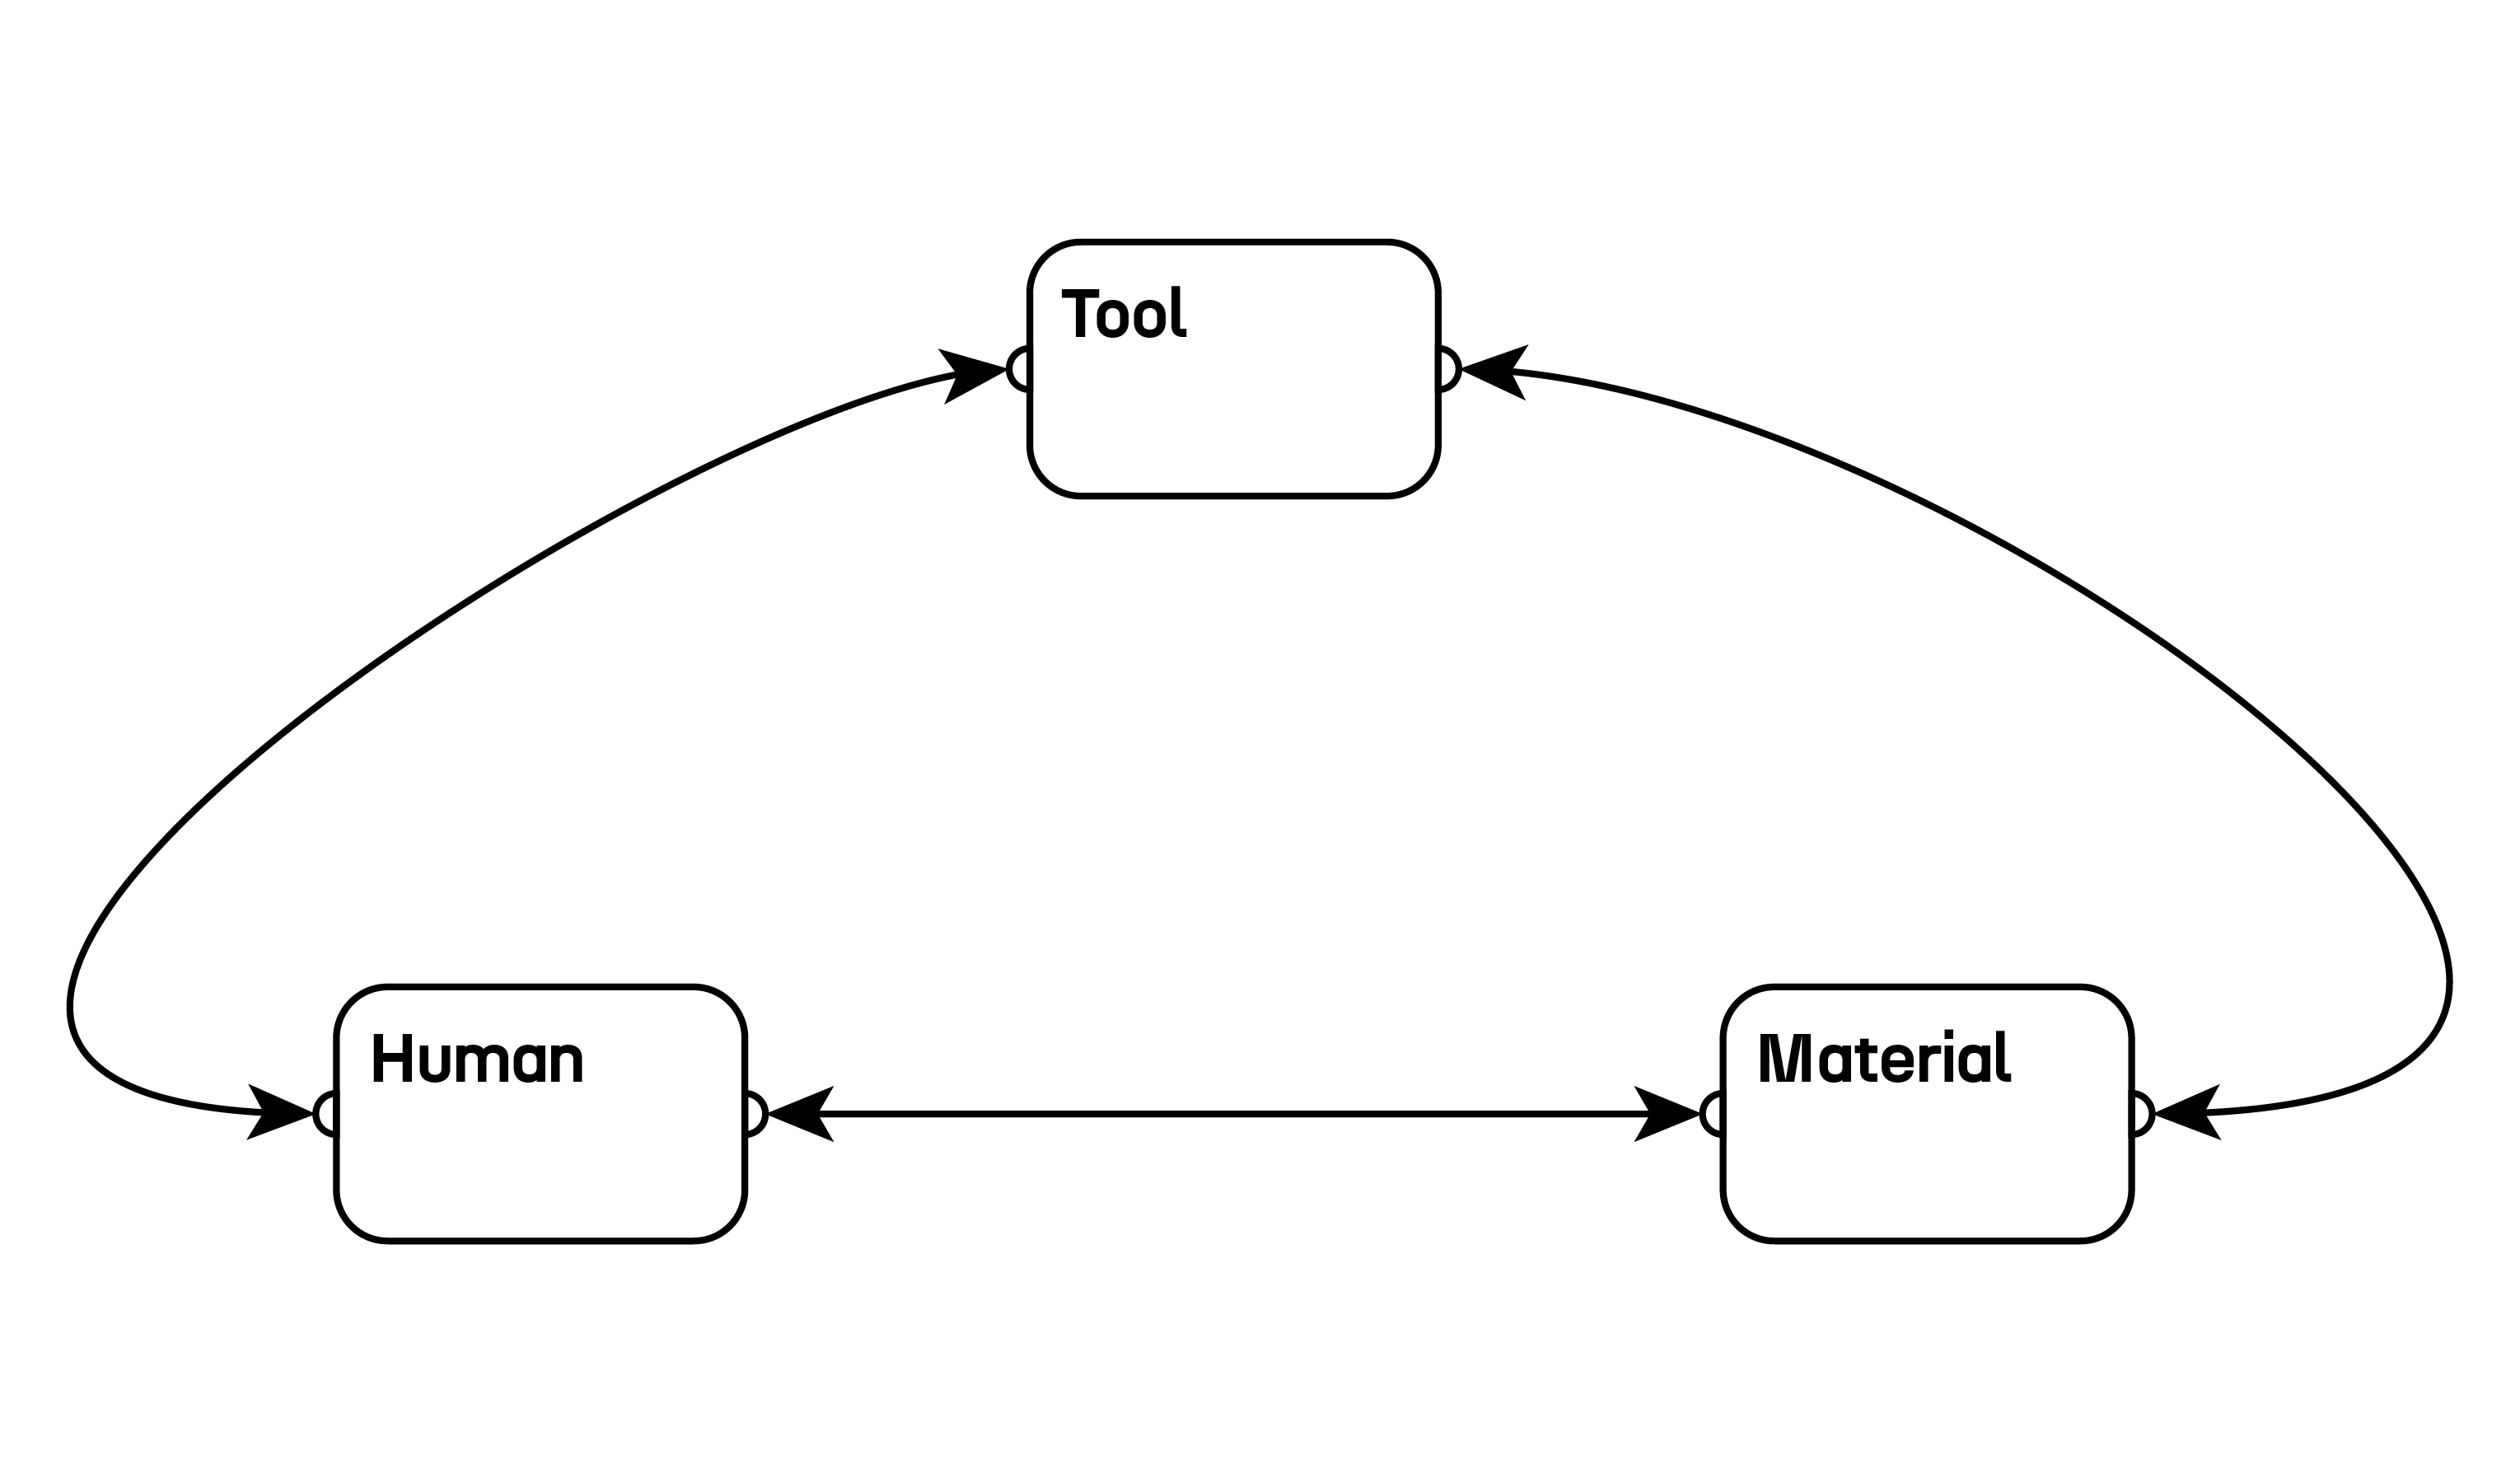
\includegraphics[width=1\textwidth]{figures/chapter1/traditional making.png}
\caption{Unified Agency diagram. Source: Author}
\label{fig:unified_agency}
\end{figure}

\subsection{Distributed Agency: Industrial and Digital Fragmentation}

The industrial transformation traced through Taylorism and later digital workflows created what this research identifies as distributed agency: a configuration where creative control becomes fragmented across separate operational domains, each governed by different systems and often different human operators. This represents a different organizational form from unified agency, not merely a technological updating of traditional craft practice.

Distributed agency operates through the "externalization of knowledge, expectation, understanding, and other elements of self" across spatial and technological domains. In digital fabrication, this externalization becomes problematic fragmentation: the craftsperson's unified practice gets distributed across discrete technological phases, each operating according to its own technical logic. Unlike the concept of "emplaced action," where place and action remain integrated, digital workflows create a "displaced action," where creative decisions become separated from their material consequences through layers of technological mediation.

Each stage of this distributed system operates as a different "place" with its own material and symbolic boundaries that shape what actions become possible. CAD environments privilege geometric precision and parametric relationships, effectively "placing" the designer within a mathematical abstraction that rewards certain types of thinking while constraining others. Toolpath generation software functions as an intermediary place governed by manufacturing efficiency and machine limitations, where the designer's intentions must conform to algorithmic optimization routines. Finally, the physical fabrication environment operates according to mechanical precision and material properties, but by this point the maker has been effectively displaced from direct engagement with these material realities. This sequential displacement across technological places creates a crisis of accountability: when creative decisions become distributed across multiple technological domains, the maker loses the direct responsiveness that is central to emplaced action.

\begin{figure}[h]
\centering
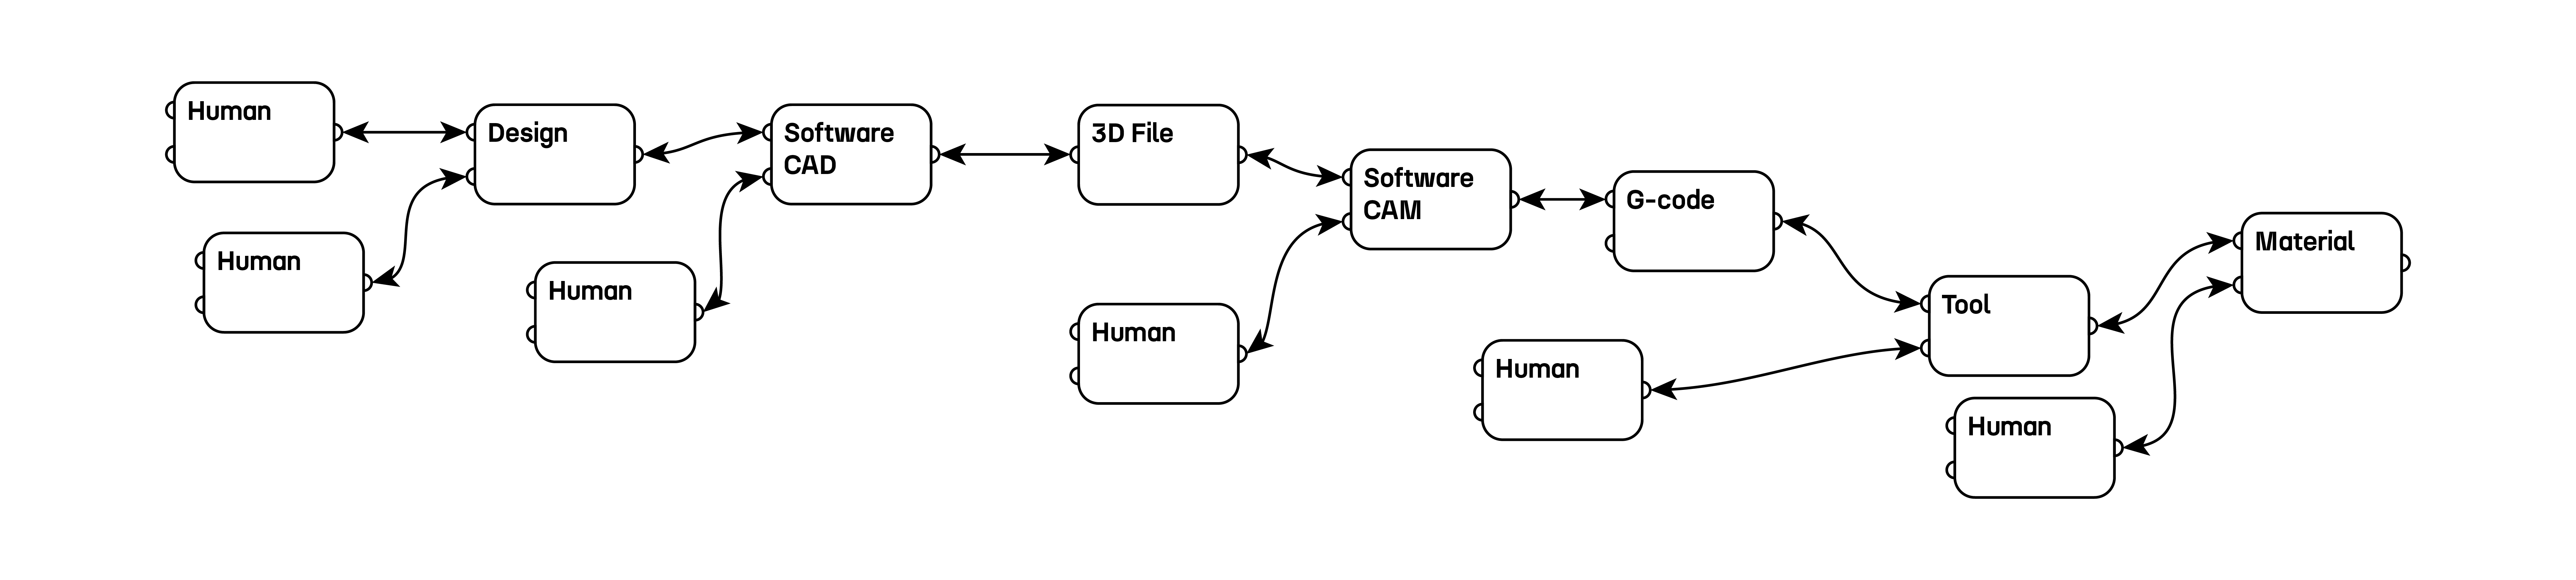
\includegraphics[width=1\textwidth]{figures/chapter1/fragmented agency.png}
\caption{Distributed Agency diagram}
\label{fig:distributed_agency}
\end{figure}

\subsection{The Loss of Adaptive Authority}

The biggest difference between unified and distributed agency lies not only in the number of technological intermediaries involved, but in the elimination of what this research identifies as adaptive authority, being the capacity for real-time modification of creative decisions based on emergent conditions. Traditional craft practice embedded this adaptive capacity throughout the making process, enabling continuous negotiation between intention and material response. Distributed agency, by contrast, concentrates adaptive authority within the initial design phase while rendering subsequent stages increasingly deterministic. Once geometric specifications are locked into CAD files and translated through manufacturing software, the system resists the kinds of responsive modifications that characterized traditional craft dialogue between maker and material.

The emergence of increasingly sophisticated computational processes, from parametric optimization to AI-generated design variations, intensifies this structural limitation. These developments may increase the sophistication of initial design exploration, but they operate within the same distributed architecture that concentrates creative authority in separate planning phases while rendering material execution increasingly automated and non-responsive.

\section{Towards Alternative Configurations}

Understanding agency as organizationally configured rather than technologically determined suggests possibilities for alternative approaches to digital fabrication. Rather than accepting the distributed model as inevitable, this research explores whether digital systems might be structured to preserve adaptive authority throughout the making process, enabling the continuous dialogue between intention and material while leveraging the capabilities of contemporary fabrication technologies.

\begin{figure}[h]
\centering
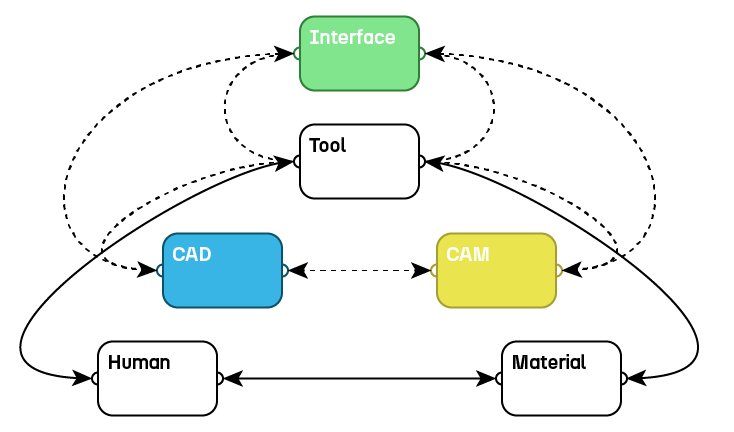
\includegraphics[width=1\textwidth]{figures/chapter1/Integrated Digital Agency.png}
\caption{Toward Integrated Digital Agency diagram. Source: Author}
\label{fig:integrated_digital_agency}
\end{figure}

\section{Reclaiming Agency Within Technological Constraints}

Out of this historical trajectory from unified craft practice through industrial fragmentation to contemporary digital workflows emerges a clear challenge: the problem facing makers today is not technological limitation but organizational structure. The tools themselves, CNC machines, 3D printers, and parametric design software, represent unprecedented capabilities for material manipulation and geometric exploration. Yet their integration within distributed agency frameworks eliminates the adaptive authority that enabled traditional craftspeople to maintain creative control throughout the making process.

Current approaches to fabrication "democratization" have focused primarily on access, making industrial machines smaller, cheaper, and more widely available, without addressing the key workflow architectures that perpetuate the separation of conception from execution. The path forward followed by this research will require a tactical appropriation: working within existing technological ecosystems while reorganizing their logic to restore the continuous dialogue between intention and material response.

Unlike the Luddites' strategic machine-breaking or the Arts \& Crafts movement's wholesale rejection of industrial methods, this approach recognizes that contemporary technological capabilities need not inevitably fragment creative agency. The challenge lies not in the machines themselves but in reorganizing how they are deployed within making workflows. The following chapters will examine how such reorganization might operate in practice, exploring pathways toward post-industrial craft practices that combine computational precision with organizational structures preserving the maker's capacity for real-time adaptation, contextual response, and embodied decision-making.